\begin{figure*}
	\centering
	\begin{tikzpicture}[
	node distance = 1cm,
	%nodes=draw,
	auto,
	scale=1.0,
	transform shape,
	triangle/.style = {regular polygon, regular polygon sides=3 },
	node rotated/.style = {rotate=180},
	border rotated/.style = {shape border rotate=180}
	]
	
	%%%%%%%%%%%%%%%%%%%%%%%%%%%%%%%%%%%%%%%%%%%%%%%%%%%%%%%%%%%%%%%%%%%%%%%%%%%%
	% 4. Word hypotheses
	\node[ 
	line width=0.2mm,
	rounded corners=2pt, 
	%rectangle, draw, 
	minimum height=7cm, 
	minimum width=\textwidth]
	at (0,0) 
	(word_hypotheses)
	{};
	
	\node[ 
	%line width=0.1mm,
	rounded corners=3pt, 
	rectangle, draw=cyan!100, line width=2pt,
	minimum height=1cm, 
	minimum width=1cm]
	at ([xshift=-22em, yshift=0em] word_hypotheses)
	(query)
	{
		
\includegraphics[width=3cm]{./images/captain.png}
	};
	
	\node[ 
	%line width=0.1mm,
	rounded corners=3pt, 
	%rectangle, draw, 
	minimum height=1cm, 
	minimum width=1cm]
	at ([xshift=+9em, yshift=0em] query.east)
	(phocnet_arch)
	{
		\includegraphics[width=5cm]{gfx/standalone_phocnet_architecture.pdf}
	};
	
	\node[ 
	%line width=0.1mm,
	rounded corners=3pt, 
	%rectangle, draw, 
	minimum height=0cm, 
	minimum width=0cm]
	at ([xshift=-0.2em, yshift=0em] phocnet_arch.east)
	(phocnet)
	{
		%\includegraphics[width=4cm]{gfx/standalone_phocnet_architecture.pdf}
	};
	
	
	\node[ 
	%line width=0.1mm,
	rounded corners=3pt, 
	%rectangle, draw, 
	minimum height=1cm, 
	minimum width=1cm]
	(cosine)
	at ([xshift=7.5em, yshift=5em] phocnet.east)
	{
		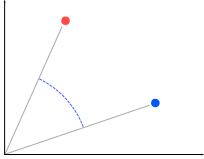
\includegraphics[width=3cm]{gfx/cosine.pdf}
	};
	
	\node[ 
	%line width=0.1mm,
	rounded corners=3pt, 
	%rectangle, draw, 
	minimum height=1cm, 
	minimum width=1cm]
	(alpha)
	at ([xshift=-2.5em, yshift=-1.75em] cosine)
	{
		\footnotesize \color{red} $\alpha$
	};
	
	\node[ 
	%line width=0.1mm,
	rounded corners=3pt, 
	%rectangle, draw, 
	minimum height=0cm, 
	minimum width=0cm]
	(cosine)
	at ([xshift=0em, yshift=0.5em] cosine.north)
	{
		\scriptsize Cosine-Similarity
	};
	
	\node[ 
	%line width=0.1mm,
	rounded corners=3pt, 
	%ellipse, draw, 
	minimum height=0.25cm, 
	minimum width=0.25cm,
	fill=cyan!100]
	(attribute_vector)
	at ([xshift=6em, yshift=7.5em] phocnet.east)
	{
	
	};
	
	\node[ 
	%line width=0.1mm,
	rounded corners=3pt, 
	ellipse, draw, 
	minimum height=2.0cm, 
	minimum width=2.0cm,
	fill=cyan!100, opacity=0.5]
	(dap_0)
	at ([xshift=6.5em, yshift=-5em] phocnet.east)
	{
%		\large $a_D$
	};
	
	\node[ 
	%line width=0.1mm,
	rounded corners=3pt, 
	ellipse, draw, 
	minimum height=2.0cm, 
	minimum width=2.0cm,
	fill=red!100, opacity=0.5]
	(dap_1)
	at ([xshift=-0.5cm, yshift=0em] dap_0.east)
	{
%		\large $a_D$
	};
	
	\node[ 
	%line width=0.1mm,
	rounded corners=3pt, 
	%ellipse, draw, 
	minimum height=2.5cm, 
	minimum width=2.5cm]
%	fill=red!100, opacity=0.5]
	(dap_2)
	at ([xshift=0.8em, yshift=0em] dap_0)
	{
		\large $P(\mathbf{q}|\mathbf{a})$
	};
	
	\node[ 
	%line width=0.1mm,
	rounded corners=3pt, 
	%rectangle, draw, 
	minimum height=2.75cm, 
	minimum width=4cm]
	(prm_frame)
	at ([xshift=0em, yshift=0.75em] dap_2)
	{
		%\normalsize Probabilistic Retrieval Model
		%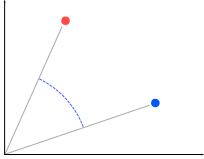
\includegraphics[width=3cm]{gfx/cosine.pdf}
	};
	
	\node[ 
	%line width=0.1mm,
	rounded corners=3pt, 
	%rectangle, draw, 
	minimum height=0cm, 
	minimum width=0cm]
	(prm)
	at ([xshift=0em, yshift=-1em] prm_frame.north)
	{
		\scriptsize Probabilistic Retrieval Model
		%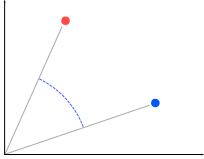
\includegraphics[width=3cm]{gfx/cosine.pdf}
	};
	
	\node[ 
	%line width=0.1mm,
	rounded corners=3pt, 
	rectangle, draw=red!100, line width=2pt,
	minimum height=0cm, 
	minimum width=0cm]
	%	fill=red!100, opacity=0.5]
	(captain)
	at ([xshift=20em, yshift=0em] phocnet.east)
	{
		\includegraphics[width=3cm]{images/captain_query.png}
	};
	
	\node[ 
	%line width=0.1mm,
	rounded corners=3pt, 
	%rectangle, draw, 
	minimum height=0cm, 
	minimum width=0cm]
	at ([xshift=0em, yshift=0em] captain.west)
	(captain_query)
	{
		%\includegraphics[width=4cm]{gfx/standalone_phocnet_architecture.pdf}
	};
	
	\node[ 
	%line width=0.1mm,
	rounded corners=3pt, 
	%ellipse, draw, 
	minimum height=0.25cm, 
	minimum width=0.25cm,
	fill=red!100]
	(query_vector)
	at ([xshift=9.95em, yshift=4.05em] phocnet.east)
	{
		
	};
	
	\draw[line width=0.75pt, -stealth] (query) -- (phocnet_arch);
	
	\draw[cyan!100, dashed, line width=0.75pt, -stealth] (phocnet) -- (attribute_vector);
	\draw[cyan!100, dashed, line width=0.75pt, -stealth] (phocnet) -- (dap_0);
	
	\draw[red!100, dashed, line width=0.75pt, -stealth] (captain_query) -- (query_vector);
	\draw[red!100, dashed, line width=0.75pt, -stealth] (captain_query) -- (dap_1);
	
%	\node[
%	line width=0.2mm,
%	rounded corners=2pt, 
%	%rectangle, draw, 
%	minimum height=3cm, 
%	minimum width=3cm]
%	at ([xshift=0em] word_hypotheses.north)
%	(cosine)
%	{
%		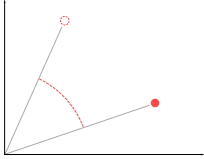
\includegraphics[width=3cm]{gfx/cosine_embedding_problem}
%	};
%	\node at ([xshift=-2.6em, yshift=-1.9em] word_hypotheses.north) {$\alpha$};
%	\node[
%	line width=0.2mm,
%	rounded corners=2pt, 
%	%rectangle, draw, 
%	minimum height=3cm, 
%	minimum width=3cm]
%	at ([xshift=10em] cosine.east)
%	{
%		\includegraphics[width=3cm]{images/captain_query}
%	};
%	%\node[anchor=south west,inner sep=0] (image) at (0,0) {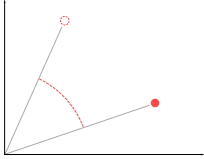
\includegraphics[width=0.28\textwidth]{gfx/cosine_embedding_problem}};
%	
%	% % % % % LENET % % % % % % %
%	\node[ 
%	rounded corners=3pt,
%	%rectangle, draw,
%	minimum height=5cm, 
%	minimum width=4.5cm]
%	at ([yshift=0em, xshift=1.75cm] word_hypotheses.west)
%	(lenet)
%	{
%		%\Large{Architectures}
%		%\includegraphics[width=5cm]{images/sift_regions_top.png}
%	};
%	\node[
%	rounded corners=3pt,
%	rectangle, draw,
%	minimum height=0.0cm, 
%	minimum width=4.2cm,
%	fill=green]
%	(conv1)
%	at ([yshift=1cm, xshift=0.0cm] lenet.south)
%	{
%		\scriptsize{1 x CONV [28,28,20]}	
%	};
%	\node[
%	rounded corners=3pt,
%	rectangle, draw,
%	minimum height=0.0cm, 
%	minimum width=4.2cm,
%	fill=orange]
%	(pool1)
%	at ([yshift=1em, xshift=0cm] conv1.north)
%	{
%		\scriptsize{POOL [2,2]}	
%	};
%	\node[
%	rounded corners=3pt,
%	rectangle, draw,
%	minimum height=0.0cm, 
%	minimum width=3.5cm,
%	fill=green]
%	(conv2)
%	at ([yshift=1em, xshift=0cm] pool1.north)
%	{
%		\scriptsize{1xCONV [14,14,50]}	
%	};
%	\node[
%	rounded corners=3pt,
%	rectangle, draw,
%	minimum height=0.0cm, 
%	minimum width=3.5cm,
%	fill=cyan!50]
%	(tpp)
%	at ([yshift=1em, xshift=0cm] conv2.north)
%	{
%		\scriptsize{TPP}	
%	};
%	\node[
%	rounded corners=3pt,
%	rectangle, draw,
%	minimum height=0.0cm, 
%	minimum width=3.0cm,
%	fill=magenta!50]
%	(fc1)
%	at ([yshift=1em, xshift=0cm] tpp.north)
%	{
%		\scriptsize{FC [500]}	
%	};
%	\node[
%	rounded corners=3pt,
%	rectangle, draw,
%	minimum height=0.0cm, 
%	minimum width=3.0cm,
%	fill=magenta!50]
%	(fc2)
%	at ([yshift=1em, xshift=0cm] fc1.north)
%	{
%		\scriptsize{FC [500]}	
%	};
%	\node[
%	rounded corners=3pt,
%	rectangle, draw,
%	minimum height=0.0cm, 
%	minimum width=3.0cm,
%	fill=yellow!50]
%	(phoc_tpp)
%	at ([yshift=1em, xshift=0cm] fc2.north)
%	{
%		\scriptsize{PHOC}	
%	};
%	% % % % % % % % % % % % % % % % % % % % % % % % % % % % % % % % %
%	
%	% % % % % TPP-PHOCNET % % % % % % % % % % % % % % % % % % % % % %
%	\node[ 
%	right = 0.0cm of lenet,
%	rounded corners=3pt,
%	%rectangle, draw,
%	minimum height=5cm, 
%	minimum width=4.5cm]
%	%at (lenet.west)
%	(tppnet)
%	{
%		%\Large{TPP-PHOCNet}
%		%\includegraphics[width=5cm]{images/sift_regions_top.png}
%	};
%	\node[
%	rounded corners=3pt,
%	rectangle, draw,
%	minimum height=0.0cm, 
%	minimum width=4.2cm,
%	fill=green]
%	(conv1)
%	at (tppnet.south)
%	{
%		\scriptsize{2 x CONV [3,3,64]}	
%	};
%	\node[
%	rounded corners=3pt,
%	rectangle, draw,
%	minimum height=0.0cm, 
%	minimum width=4.2cm,
%	fill=orange]
%	(pool1)
%	at ([yshift=1em, xshift=0cm] conv1.north)
%	{
%		\scriptsize{POOL [2,2]}	
%	};
%	\node[
%	rounded corners=3pt,
%	rectangle, draw,
%	minimum height=0.0cm, 
%	minimum width=3.5cm,
%	fill=green]
%	(conv2)
%	at ([yshift=1em, xshift=0cm] pool1.north)
%	{
%		\scriptsize{2xCONV [3,3,64]}	
%	};
%	\node[
%	rounded corners=3pt,
%	rectangle, draw,
%	minimum height=0.0cm, 
%	minimum width=3.5cm,
%	fill=orange]
%	(pool2)
%	at ([yshift=1em, xshift=0cm] conv2.north)
%	{
%		\scriptsize{POOL [2,2]}	
%	};
%	\node[
%	rounded corners=3pt,
%	rectangle, draw,
%	minimum height=0.0cm, 
%	minimum width=3.0cm,
%	fill=green]
%	(conv3)
%	at ([yshift=1em, xshift=0cm] pool2.north)
%	{
%		\scriptsize{6xCONV [3,3,256]}	
%	};
%	\node[
%	rounded corners=3pt,
%	rectangle, draw,
%	minimum height=0.0cm, 
%	minimum width=3.0cm,
%	fill=green]
%	(conv4)
%	at ([yshift=1em, xshift=0cm] conv3.north)
%	{
%		\scriptsize{6xCONV [3,3,256]}	
%	};
%	\node[
%	rounded corners=3pt,
%	rectangle, draw,
%	minimum height=0.0cm, 
%	minimum width=3.0cm,
%	fill=cyan!50]
%	(tpp)
%	at ([yshift=1em, xshift=0cm] conv4.north)
%	{
%		\scriptsize{TPP}	
%	};
%	\node[
%	rounded corners=3pt,
%	rectangle, draw,
%	minimum height=0.0cm, 
%	minimum width=3.0cm,
%	fill=magenta!50]
%	(fc1)
%	at ([yshift=1em, xshift=0cm] tpp.north)
%	{
%		\scriptsize{FC [4096]}	
%	};
%	\node[
%	rounded corners=3pt,
%	rectangle, draw,
%	minimum height=0.0cm, 
%	minimum width=3.0cm,
%	fill=magenta!50]
%	(fc2)
%	at ([yshift=1em, xshift=0cm] fc1.north)
%	{
%		\scriptsize{FC [4096]}	
%	};
%	\node[
%	rounded corners=3pt,
%	rectangle, draw,
%	minimum height=0.0cm, 
%	minimum width=3.0cm,
%	fill=yellow!50]
%	(phoc_tpp)
%	at ([yshift=1em, xshift=0cm] fc2.north)
%	{
%		\scriptsize{PHOC}	
%	};
	
	% % % % % % % % % % % % % % % % % % % % % % % % % % % % % % % % % %
	
	% % % % % RESNET % % % % % % %
%	\node[ 
%	right = 0.0cm of tppnet,
%	rounded corners=3pt,
%	%rectangle, draw,
%	minimum height=5cm, 
%	minimum width=4.5cm]
%	%at (lenet.west)
%	(resnet)
%	{
%		\Large{PHOCResNet}
%		%\includegraphics[width=5cm]{images/sift_regions_top.png}
%	};
%	\node[
%	rounded corners=3pt,
%	rectangle, draw,
%	minimum height=0.0cm, 
%	minimum width=4.2cm,
%	fill=green!50]
%	(conv1)
%	at ([yshift=0.0cm, xshift=0.0cm] resnet.south)
%	{
%		\tiny{1 x CONV [7,7,64]}	
%	};
%	\node[
%	rounded corners=3pt,
%	rectangle, draw,
%	minimum height=0.0cm, 
%	minimum width=4.2cm,
%	fill=orange!50]
%	(pool1)
%	at ([yshift=1em, xshift=0cm] conv1.north)
%	{
%		\tiny{POOL [2,2]}	
%	};
%	\node[
%	rounded corners=3pt,
%	rectangle, draw,
%	minimum height=2.5cm, 
%	minimum width=3.5cm,
%	fill=green!10]
%	(resnetblock)
%	at ([yshift=4em, xshift=0cm] pool1.north)
%	{
%		%empty	
%	};
%	\node[
%	rounded corners=3pt,
%	rectangle, draw,
%	minimum height=0.0cm, 
%	minimum width=1.5cm,
%	fill=green!50]
%	(block_conv1)
%	at ([yshift=1.85em, xshift=0cm] resnetblock.south)
%	{
%		\tiny{CONV [1,1,64]}	
%	};
%	\node[
%	rounded corners=3pt,
%	rectangle, draw,
%	minimum height=0.0cm, 
%	minimum width=1.5cm,
%	fill=green!50]
%	(block_conv2)
%	at ([yshift=1.1em, xshift=0cm] block_conv1.north)
%	{
%		\tiny{CONV [3,3,64]}	
%	};
%	\node[
%	rounded corners=3pt,
%	rectangle, draw,
%	minimum height=0.0cm, 
%	minimum width=1.5cm,
%	fill=green!50]
%	(block_conv3)
%	at ([yshift=1.1em, xshift=0cm] block_conv2.north)
%	{
%		\tiny{CONV [1,1,256]}	
%	};
	
%	\node[
%	%rounded corners=3pt,
%	%ellipse, draw,
%	minimum height=-1.0cm, 
%	minimum width=-1.0cm]
%	(start)
%	at ([yshift=-0.75em, xshift=0cm] block_conv1.south)
%	{
%			\Huge{.}
%	};
%	
%	\node[
%	%rounded corners=3pt,
%	%ellipse, draw,
%	minimum height=-1.0cm, 
%	minimum width=-1.0cm]
%	(end)
%	at ([yshift=0.75em, xshift=0cm] block_conv3.north)
%	{
%			\Huge{.}
%	};
%	
%	\node[
%	rounded corners=3pt,
%	rectangle, draw,
%	minimum height=0.0cm, 
%	minimum width=3.5cm,
%	fill=cyan!50]
%	(tpp_resnet)
%	at ([yshift=1em, xshift=0cm] resnetblock.north)
%	{
%		\tiny{TPP}	
%	};
%	\node[
%	rounded corners=3pt,
%	rectangle, draw,
%	minimum height=0.0cm, 
%	minimum width=3.0cm,
%	fill=magenta!50]
%	(fc1)
%	at ([yshift=1em, xshift=0cm] tpp_resnet.north)
%	{
%		\tiny{FC [4096]}	
%	};
%	\node[
%	rounded corners=3pt,
%	rectangle, draw,
%	minimum height=0.0cm, 
%	minimum width=3.0cm,
%	fill=magenta!50]
%	(fc2)
%	at ([yshift=1em, xshift=0cm] fc1.north)
%	{
%		\tiny{FC [4096]}	
%	};
%	\node[
%	rounded corners=3pt,
%	rectangle, draw,
%	minimum height=0.0cm, 
%	minimum width=3.0cm,
%	fill=yellow!50]
%	(phoc_tpp)
%	at ([yshift=1em, xshift=0cm] fc2.north)
%	{
%		\tiny{PHOC}	
%	};
%	
%	
%	\draw[line width=0.25mm] (start) arc [x radius = 1.5cm, y radius = 1.05cm, start angle = -90,end angle = +90] (end);
%	
%	\draw[line width=0.27mm] (pool1) -- (block_conv1);
%	
%	\draw[line width=0.27mm] (block_conv1) -- (block_conv2);
%	
%	\draw[line width=0.27mm] (block_conv2) -- (block_conv3);
%	
%	\draw[line width=0.27mm] (block_conv3) -- (tpp_resnet);
	
	% % % % % % % % % % % % % % % % % % % % % % % % % % % % % % % % %

	
%	% % % % % PHOCDenseNet % % % % % % %
%	\node[ 
%	right = 0.0cm of resnet,
%	rounded corners=3pt,
%	%rectangle, draw,
%	minimum height=5cm, 
%	minimum width=4.5cm]
%	%at (lenet.west)
%	(densenet)
%	{
%		%\Large{PHOCResNet}
%		%\includegraphics[width=5cm]{images/sift_regions_top.png}
%	};
%	\node[
%	rounded corners=3pt,
%	rectangle, draw,
%	minimum height=0.0cm, 
%	minimum width=4.2cm,
%	fill=green!50]
%	(dense_conv1)
%	at ([yshift=0.0cm, xshift=0.0cm] densenet.south)
%	{
%		\tiny{1 x CONV [7,7,64]}	
%	};
%	\node[
%	rounded corners=3pt,
%	rectangle, draw,
%	minimum height=0.0cm, 
%	minimum width=4.2cm,
%	fill=orange!50]
%	(dense_pool1)
%	at ([yshift=0.75em, xshift=0cm] dense_conv1.north)
%	{
%		\tiny{POOL [2,2]}	
%	};
%	\node[
%	rounded corners=3pt,
%	rectangle, draw,
%	minimum height=2.5cm, 
%	minimum width=3.5cm,
%	fill=green!10]
%	(denseblock)
%	at ([yshift=4em, xshift=0cm] dense_pool1.north)
%	{
%		\tiny{1xCONV [14,14,50]}	
%	};
%	\node[
%	rounded corners=3pt,
%	rectangle, draw,
%	minimum height=0.0cm, 
%	minimum width=1.5cm,
%	fill=green!50]
%	(denseblock_conv1)
%	at ([yshift=1.35em, xshift=0cm] denseblock.south)
%	{
%		\tiny{CONV [1,1,64]}	
%	};
%	\node[
%	rounded corners=3pt,
%	rectangle, draw,
%	minimum height=0.0cm, 
%	minimum width=1.5cm,
%	fill=green!50]
%	(denseblock_conv2)
%	at ([yshift=1.5em, xshift=0cm] denseblock_conv1.north)
%	{
%		\tiny{CONV [3,3,64]}	
%	};
%	\node[
%	rounded corners=3pt,
%	rectangle, draw,
%	minimum height=0.0cm, 
%	minimum width=1.5cm,
%	fill=green!50]
%	(denseblock_conv3)
%	at ([yshift=1.5em, xshift=0cm] denseblock_conv2.north)
%	{
%		\tiny{CONV [1,1,256]}	
%	};
%	
%	\node[
%	%rounded corners=3pt,
%	%ellipse, draw,
%	minimum height=-1.0cm, 
%	minimum width=-1.0cm]
%	(dense_start)
%	at ([yshift=-0.5em, xshift=0cm] denseblock_conv1.south)
%	{
%		\Huge{.}
%	};
%	
%	\node[
%	%rounded corners=3pt,
%	%ellipse, draw,
%	minimum height=-1.0cm, 
%	minimum width=-1.0cm]
%	(dense_node_1)
%	at ([yshift=0.5em, xshift=0cm] denseblock_conv1.north)
%	{
%		\Huge{.}
%	};
%	
%	\node[
%	%rounded corners=3pt,
%	%ellipse, draw,
%	minimum height=-1.0cm, 
%	minimum width=-1.0cm]
%	(dense_node_2)
%	at ([yshift=0.5em, xshift=0cm] denseblock_conv2.north)
%	{
%		\Huge{.}
%	};
%	
%	\node[
%	%rounded corners=3pt,
%	%ellipse, draw,
%	minimum height=-1.0cm, 
%	minimum width=-1.0cm]
%	(dense_end)
%	at ([yshift=0.6em, xshift=0cm] denseblock_conv3.north)
%	{
%		\Huge{.}
%	};
%	
%	\node[
%	rounded corners=3pt,
%	rectangle, draw,
%	minimum height=0.0cm, 
%	minimum width=3.5cm,
%	fill=cyan!50]
%	(tpp_densenet)
%	at ([yshift=1em, xshift=0cm] denseblock.north)
%	{
%		\tiny{TPP}	
%	};
%	\node[
%	rounded corners=3pt,
%	rectangle, draw,
%	minimum height=0.0cm, 
%	minimum width=3.0cm,
%	fill=magenta!50]
%	(dense_fc1)
%	at ([yshift=1em, xshift=0cm] tpp_densenet.north)
%	{
%		\tiny{FC [4096]}	
%	};
%	\node[
%	rounded corners=3pt,
%	rectangle, draw,
%	minimum height=0.0cm, 
%	minimum width=3.0cm,
%	fill=magenta!50]
%	(dense_fc2)
%	at ([yshift=1em, xshift=0cm] dense_fc1.north)
%	{
%		\tiny{FC [4096]}	
%	};
%	\node[
%	rounded corners=3pt,
%	rectangle, draw,
%	minimum height=0.0cm, 
%	minimum width=3.0cm,
%	fill=yellow!50]
%	(dense_phoc_tpp)
%	at ([yshift=1em, xshift=0cm] dense_fc2.north)
%	{
%		\tiny{PHOC}	
%	};
%	
%	
%	\draw[line width=0.25mm] (dense_start) arc [x radius = 1.5cm, y radius = 0.375cm, start angle = -90,end angle = +90] (dense_node_1);
%	\draw[line width=0.25mm] (dense_node_1) arc [x radius = 1.5cm, y radius = 0.375cm, start angle = -90,end angle = +90] (dense_node_2);
%	\draw[line width=0.25mm] (dense_node_2) arc [x radius = 1.5cm, y radius = 0.375cm, start angle = -90,end angle = +90] (dense_end);
%	
%	\draw[line width=0.25mm] (dense_start) arc [x radius = 1.5cm, y radius = 0.75cm, start angle = -90,end angle = +90] (dense_node_2);
%	\draw[line width=0.25mm] (dense_node_1) arc [x radius = 1.5cm, y radius = 0.75cm, start angle = -90,end angle = +90] (dense_node_2);
%
%	\draw[line width=0.25mm] (dense_start) arc [x radius = 1.5cm, y radius = 1.11cm, start angle = -90,end angle = +90] (dense_node_2);
%		
%	\draw[line width=0.27mm] (dense_pool1) -- (denseblock_conv1);
%	
%	\draw[line width=0.27mm] (denseblock_conv1) -- (denseblock_conv2);
%	
%	\draw[line width=0.27mm] (denseblock_conv2) -- (denseblock_conv3);
%	
%	\draw[line width=0.27mm] (denseblock_conv3) -- (tpp_densenet);
	
	% % % % % % % % % % % % % % % % % % % % % % % % % % % % % % % % %
	
	%%%%%%%%%%%%%%%%%%%%%%%%%%%%%%%%%%%%%%%%%%%%%%%%%%%%%%%%%%%%%%%%%%%%%%%%%%%%
	
	\end{tikzpicture}
	\caption{Overview of the attribute prediction framework using a CNN. The CNN is trained to predict a desired attribute prepresentation generated from the annotation. Word spotting can then be performed either by the Probabilistic Retrieval Model obtaining probabilities for each test image given a query or in the embedding space through a simple nearest neighbor search using the cosine similarity as the distance metric.}
	\label{fig:method_overview}
\end{figure*}
